\section{Namespace: Data laget}

\begin{figure}[H]
	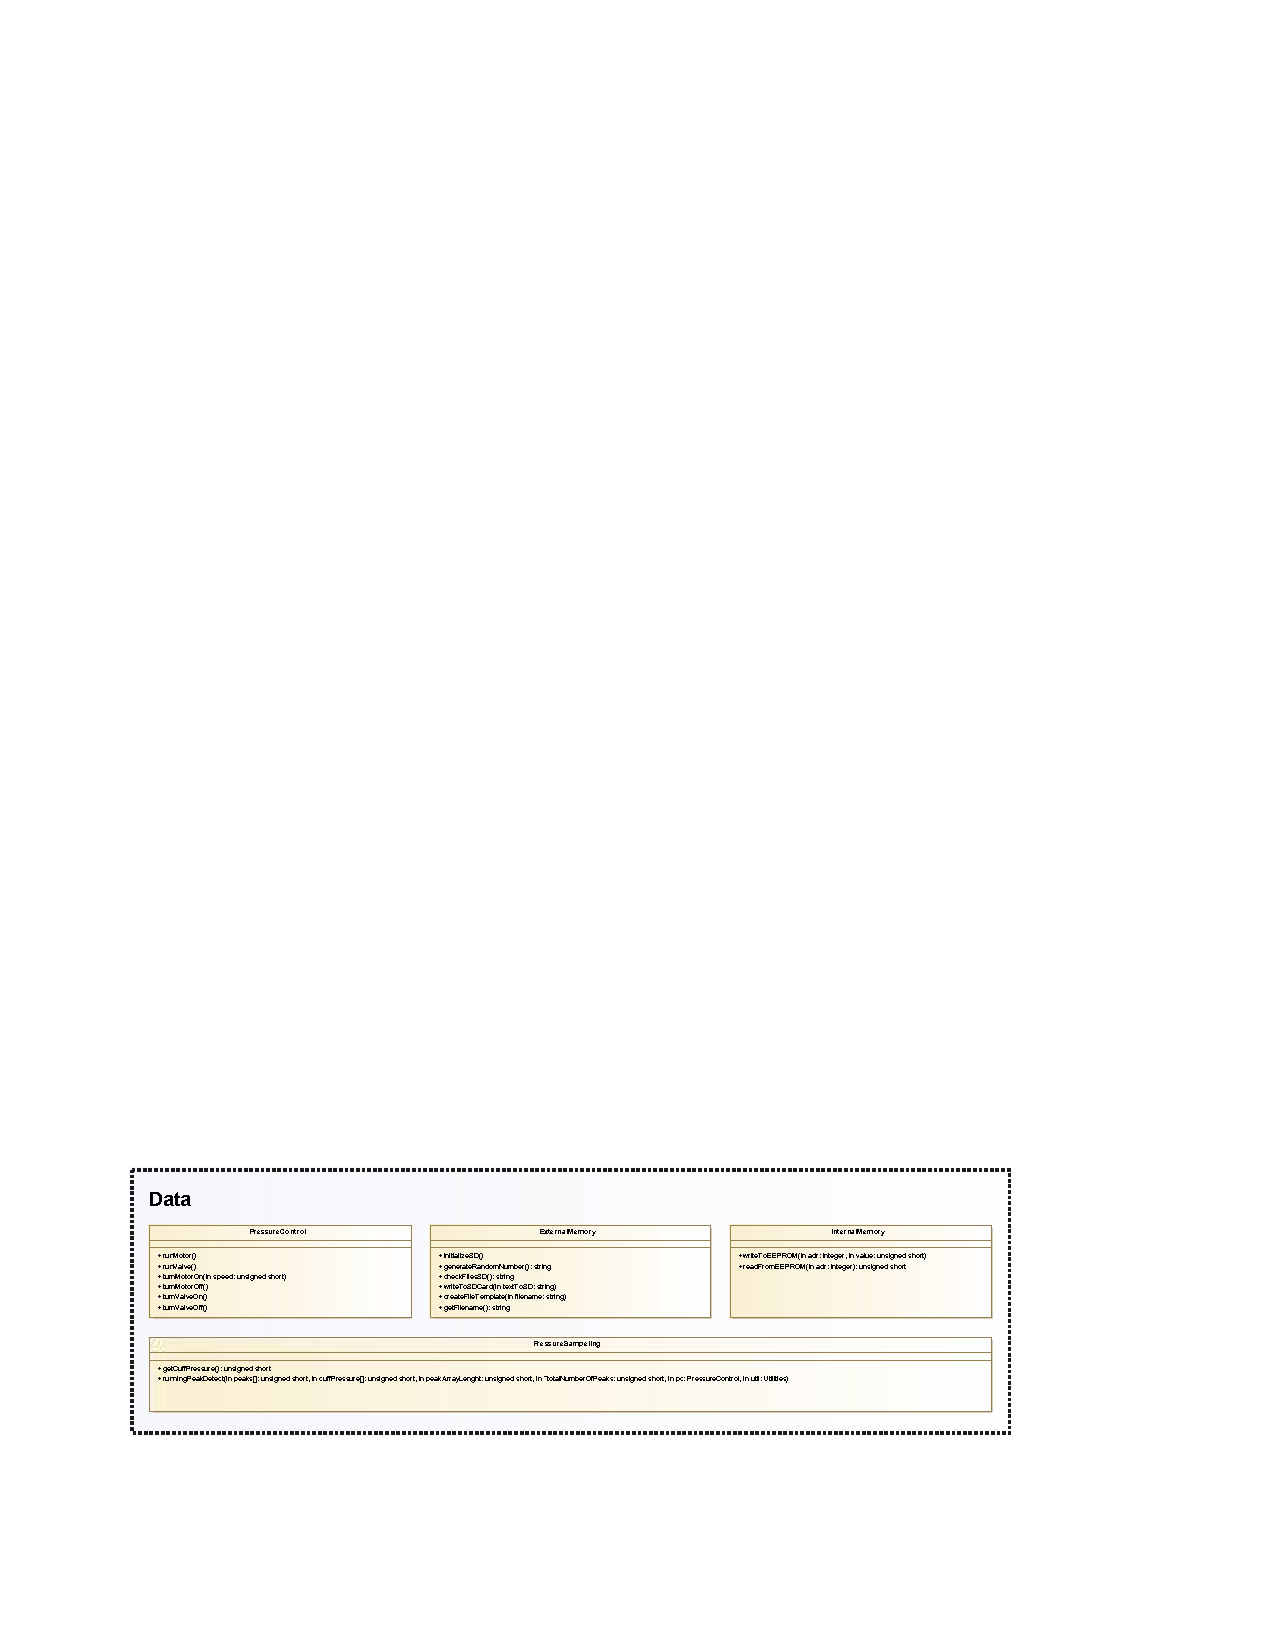
\includegraphics[ width=\textwidth]{Implementeringsdokument/klassediagram_Data-crop.pdf}
	\caption{Klasse diagram over namespacet data}\label{fig:classDiagramData}
\end{figure}

\subsection{Klasse: PressureControl}

\subsubsection{Metode: runMotor()}
\textbf{Parameter: } 
\\ \textbf{Returtype: } \textit{void}
\\ \textbf{Beskrivelse: }  Funktionen starter motoren og lader den kører ved 100\% duty cycle indtil interrupt knappen på pin 18 ikke længere leverer en høj.

\subsubsection{Metode: runValve()}
\textbf{Parameter: } 
\\ \textbf{Returtype: } \textit{void}
\\ \textbf{Beskrivelse: }  Funktionen åbner for ventilen og lader den kører ved 100\% duty cycle indtil interrupt knappen på pin 19 ikke længere leverer en høj.

\subsubsection{Metode: turnMotorOn()}
\textbf{Parameter: } 
\\ \textbf{Returtype: } \textit{void}
\\ \textbf{Beskrivelse: } Funktionen tænder for motoren med den hastighed, angivet i parameteren (0-255).

\subsubsection{Metode: turnMotorOff()}
\textbf{Parameter: } 
\\ \textbf{Returtype: } \textit{void}
\\ \textbf{Beskrivelse: }   Funktionen stopper for motoren ved at sætte pin 3 lav.

\subsubsection{Metode: turnValveOn()}
\textbf{Parameter: } 
\\ \textbf{Returtype: } \textit{void}
\\ \textbf{Beskrivelse: }  Funktionen åbner for ventilen ved at sætte pin 11 høj.

\subsubsection{Metode: turnValveOff()}
\textbf{Parameter: } 
\\ \textbf{Returtype: } \textit{void}
\\ \textbf{Beskrivelse: }  Funktionen lukker for ventilen ved at sætte pin 11 lav.

\subsection{Klasse: ExternalMemory}
Denne klasse gør brug af to arduino biblioteker hhv. SD og SPI.  De to biblioteker muliggøre kommunikation med SD kortet via en SPI forbindelse. 

\subsubsection{Metode: initializeSDCard()}
\textbf{Parameter: } 
\\ \textbf{Returtype: } \textit{void}
\\ \textbf{Beskrivelse: }  Simple metode der starter kommunikation med SD kortet og køre metoden\textit{ checkFilesSD()} (Se \ref{title:checkFiles})

\subsubsection{Metode: generateRandomNumber()} \label{title:RandomNumber}
\textbf{Parameter: } 
\\ \textbf{Returtype: } \textit{String}
\\ \textbf{Beskrivelse: }  Denne metode generer et 6-cifret tilfældigt nummer. Arduinos indbyggede funktion \textit{random()} laver et tilfældigt nummer i det interval man specificerer, men den generer dem i samme rækkefølge hver gang. For at gøre nummeret “mere tilfældigt” styres rækkefølgen af de generede numre af værdien fra en analog port, som svæver. Den tilfældige HEX værdi skal bruges som ID for patienten der modtager konditioneringsbehandling.
\begin{lstlisting}
	randomSeed(analogRead(A5)); 
	long randNumber = random(100000, 999999); 
	String randNumberHEX = String(String(randNumber, HEX) +	".csv");
	return randNumberHEX; 
\end{lstlisting}
Når der er lavet et 6-cifre tilfældigt nummer, bliver dette konverteret til en HEX, så værdien nu indeholder tal mellem 0-9 og bogstaver mellem A-F. Denne værdi bliver returneret som en string. 

\subsubsection{Metode: checkFilesSD()} \label{title:checkFiles}
\textbf{Parameter: } \textit{File dir, String val}
\\ \textbf{Returtype: } \textit{String}
\\ \textbf{Beskrivelse: }  Metode der kontrollere alle filer på SD kortet. Hver gang der findes en fil, tjekkes der for om de sidste 4 karakterer matcher med karaktererne “.csv”. Hvis den fundne fil matcher dette, bliver hele filnavnet gemt i en variable og returneret. Hvis der ikke findes et fil med endelsen ".csv" køres metoden \textit{generateRandomNumber} og der oprettes en ny .csv fil. 
\begin{lstlisting}
String tempName, tempType, finalFile;
String valToCheck = ".csv";
File root = SD.open("/"); //Tell the method where to look on the SD card
while(true){
File entry = root.openNextFile();

//When a file is found, check the last four characters
tempName = entry.name();
tempType = tempName.substring(5,9);

//If a .csv is found
if(tempType.equalsIgnoreCase(valToCheck)){
Serial.print("*** A file was found with name: "); Serial.println(tempName);
finalFile = tempName;
break;
}
//If no file was found, creates a file
if(!tempType.equalsIgnoreCase(valToCheck) && !entry){
String newFileName = generateRandomNumber();
//Create a new file with the random HEX as filename and generate a new header
Serial.print("*** A new file was created: "); Serial.println(tempName);
createFileTemplate(newFileName);
finalFile = newFileName;
break;
}
entry.close();
}
return finalFile;
}
\end{lstlisting}
For at sikre at alle filer på SD kortet kontrolleres, kører metode i et loop, som kun brydes hvis den finder en .csv fil, eller hvis alle filer er kontrolleret og der ikke blev fundet en .csv fil. 

\subsubsection{Metode: createFileTemplate()} \label{title:createTemplate}
\textbf{Parameter: } \textit{}
\\ \textbf{Returtype: } \textit{String filename}
\\ \textbf{Beskrivelse: }  Når der skal laves en ny fil på SD-kortet, skal der skrives en header til hver kolonne i .csv filen. Denne metode modtager et filnavn, som den åbner og skriver i en header til. 

\subsubsection{Metode: writeToSDCard()}
\textbf{Parameter: } \textit{String textToSD}
\\ \textbf{Returtype: } \textit{void}
\\ \textbf{Beskrivelse: }  Denne metode modtager en tekst, som den skriver til .csv filen på SD kortet.

\subsubsection{Metode: getFilename()}
\textbf{Parameter: }\textit{}
\textbf{Returtype: } \textit{String}
\textbf{Beskrivelse: } Simple metode der returnere en lokal variable, som indeholder navnet på den fundne .csv fil.

\subsection{Klasse: InternalMemory}
Klassen gør brug af bibliotektet \textit{EEPROM}, dette bibliotek gør kommunikation muligt med EEPROMen. 

\subsubsection{Metode: writeToEEPROM()}
\textbf{Parameter: } \textit{int adr, unsigned short value}
\\ \textbf{Returtype: } \textit{void}
\\ \textbf{Beskrivelse: }  Simple metode der skriver \textit{value} til adressen \textit{adr} på EEPROM.

\subsubsection{Metode: readFromEEPROM()}
\textbf{Parameter: } \textit{int adr}
\\ \textbf{Returtype: } \textit{unsigned short}
\\ \textbf{Beskrivelse: }  Metode der læser værdien på adressen \textit{adr} på EEPROM. 

\subsection{Klasse: PressureSampling}

\subsubsection{Metode: getCuffPressure()}
\textbf{Parameter: } 
\\ \textbf{Returtype: } \textit{unsigned short }
\\ \textbf{Beskrivelse: } Returnerer det aktuelle tryk i manchetten ved at sample 10 gange og tage middelværdien.

\subsubsection{Metode: runningPeakDetect())}
\textbf{Parameter: } \textit{unsigned short peaks[], unsigned short cuffPressure[],unsigned short peakArrayLength, unsigned short *totalNumberOfPeaks, PressureControl pc, Utilities util}
\\ \textbf{Returtype: } \textit{void}
\\ \textbf{Beskrivelse: } Denne metode anvender en pointer til et array med peak værdier, et array med manchettryk værdier, en variabel med værdien tilsvarende længden af de to arrays, samt en pointer til en variabel hvor metoden skriver hvor mange peaks, som der er blevet fundet. De sidste parametre er bare objekter af de klasser som indeholder metoder der skal bruges i runningPeakDetect().
Metoden sampler et sample ad gangen (i alt 13) og tjekker om værdien er højerer end middelværdien af de 6 samples før og de 6 samples efter. Hvis sample x(n-6) er størst og er højerer end thresholdværdien for et detekteret puls signal, så gemmes peak værdien i “peaks[]” og manchettrykket i “cuffPressure[]”.
\begin{lstlisting}
	if(timestamp<millis()-400 && n6>thresshold && (n12+n11+n10+n9+n8+n7)/6 < n6 && (n+n1+n2+n3+n4+n5)/6 < n6)
	{
	peaks[tNOPeaks] = n6;
	cuffPressure[tNOPeaks] = getCuffPressure();
	tNOPeaks++;
	}
\end{lstlisting}
If sætningen sikre også at peaks har mindst 400ms i afstand. Ved at have minimum afstand mellem detekteret pulssignal sikres at flere peaks på en puls ikke detekteres. Metoden fortsætter med at sample ind til manchet trykket når under 40mmHg, hvorefter den stopper. 
\begin{lstlisting}
	while(currentPressure > util.mmHgToRaw(40))
	{
\end{lstlisting}
Fordi de to arrays, som indeholder henholdsvis peaks og cuffpressure er prealokeret i hukommelsen, sættes de resterende ubrugte pladser = NULL. Dette sikrer at de værdier, som ellers måtte være liggende i hukommelsen ikke bliver forvekslet med en peak amplitude. 
\begin{lstlisting}
	for(i = tNOPeaks; i < peakArrayLength; i++)
	{
		peaks[i] = NULL;
		cuffPressure[i] = NULL;
	}
\end{lstlisting}
Til sidst lukkes den resterende luft ud af manchetten, altså de sidste 40mmHg.
